\documentclass{article}
\usepackage{assignment_preamble}

\title{Lab 3}
\author{Ravi Kini}
\date{November 12, 2023}

\begin{document}

\maketitle

\repository{https://github.com/ravidosa/notes/tree/main/academics/assignments/code/phy112l_lab3}

\problem
The energy of an atom in a box with $x$-, $y$-, and $z$-velocities $v_x, v_y, v_z$ can be expressed as:

\begin{equation}
    E(v_x, v_y, v_z) = \frac{1}{2}mv^2 = \frac{1}{2}(v_x^2 + v_y^2 + v_z^2)
\end{equation}
Including the gravitational potential, if the atom has height $z$, the energy can be expressed as:

\begin{equation}
    E(v_x, v_y, v_z, z) = \frac{1}{2}mv^2 + mgz = \frac{1}{2}(v_x^2 + v_y^2 + v_z^2) + mgz
\end{equation}
For an argon atom in a $100$ \unit[per-mode = symbol]{\degree\kelvin} box:

\begin{equation}
    \begin{split}
        \frac{k_B T}{E(v = 100~\unit[per-mode = symbol]{\meter\per\second}) - E_0} & = \frac{1.38 \cdot 10^{-23} \cdot 300}{\frac{1}{2} \cdot 6.64 \cdot 10^{-26} \cdot 100^2} \approx 12.470 \\
        \frac{k_B T}{E(v = 1000~\unit[per-mode = symbol]{\meter\per\second}) - E_0} & = \frac{1.38 \cdot 10^{-23} \cdot 300}{\frac{1}{2} \cdot 6.64 \cdot 10^{-26} \cdot 1000^2} \approx 0.125
    \end{split}
\end{equation} 
Both the state where the atom has velocity $v = 100$ \unit[per-mode = symbol]{\meter\per\second} and velocity $v = 1000$ \unit[per-mode = symbol]{\meter\per\second} are accessible as neither ratio is negligible in comparison to $1$, although the state with $v = 100$ \unit[per-mode = symbol]{\meter\per\second} is more likely. Comparing the probability of the argon atom being found at $z = 0$ \unit[per-mode = symbol]{\meter} to the probabilities of the argon atom being found at $z = 10, 10^4$ \unit[per-mode = symbol]{\meter}:

\begin{equation}
    \begin{split}
        \frac{p(z = 10~\unit[per-mode = symbol]{\meter})}{p(z = 0~\unit[per-mode = symbol])} & = \frac{e^{-\frac{\frac{1}{2}mv^2 + mg(10)}{k_B T}}}{e^{-\frac{\frac{1}{2}mv^2 + mg(0)}{k_B T}}} \\
        & = e^{-\frac{10mg}{k_B T}} \\
        & = e^{-\frac{10 \cdot 6.64 \cdot 10^{-26} \cdot 9.8}{1.38 \cdot 10^{-23} \cdot 300}} \approx 0.998 \\
        \frac{p(z = 10^4~\unit[per-mode = symbol]{\meter})}{p(z = 0~\unit[per-mode = symbol])} & = \frac{e^{-\frac{\frac{1}{2}mv^2 + mg(10^4)}{k_B T}}}{e^{-\frac{\frac{1}{2}mv^2 + mg(0)}{k_B T}}} \\
        & = e^{-\frac{10^4mg}{k_B T}} \\
        & = e^{-\frac{10^4 \cdot 6.64 \cdot 10^{-26} \cdot 9.8}{1.38 \cdot 10^{-23} \cdot 300}} \approx 0.208 \\
    \end{split}
\end{equation}
On Mount Everest (elevation $z \approx 10^4~\unit[per-mode = symbol]{\meter}$), the air is around $\frac{1}{3}$ as thin as it is at sea level, which is higher than the result found using the Boltzmann distribution.

\clearpage

\problem
\subsection*{Part (a)}
A ten site Ising model system has $2^{10} = 1024$ states.
\subsection*{Part (b)}
${10 \choose 10} = 1$ state has ten up and zero down.
\subsection*{Part (c)}
${10 \choose 9} = 10$ states have nine up and one down.
\subsection*{Part (d)}
${10 \choose 8} = 45$ states have eight up and two down.
\subsection*{Part (e)} Calculating the number of states for all possible partitions into "up" and "down":
\begin{center}
\begin{tabular}{|c|c|c|}
    \hline
    Up & Down & Multiplicity \\
    \hline
    10 & 0 & 1 \\
    \hline
    9 & 1 & 10 \\
    \hline
    8 & 2 & 45 \\
    \hline
    7 & 3 & 120 \\
    \hline
    6 & 4 & 210 \\
    \hline
    5 & 5 & 252 \\
    \hline
    4 & 6 & 210 \\
    \hline
    3 & 7 & 120 \\
    \hline
    2 & 8 & 45 \\
    \hline
    1 & 9 & 10 \\
    \hline
    0 & 10 & 1 \\
    \hline
\end{tabular}
\end{center}
\subsection*{Part (f)}
Summing the multipliciies for each of the possible partitions:
\begin{equation}
    \begin{split}
        2(1 + 10 + 45 + 120 + 210) + 252 & = 1024
    \end{split}
\end{equation}
The numbers sum to the total states calculated in (a).

\clearpage

\problem
The program outputs:
\begin{center}
    \begin{tabular}{|c|c|}
        \hline
        Quantity & Value \\
        \hline
        $\langle E \rangle$ & -3.683793973107949  \\
        \hline
        $C$ & 1.4162919967169392 \\
        \hline
        $S$ & 6.154960904946007 \\
        \hline
        $F$ & -17.840204054483763 \\
        \hline
    \end{tabular}
\end{center}

\clearpage

\problem
Figure \ref{fig:fig1} is a plot of $\langle E \rangle, C, S, F$ vs. $T$ for $J = 1$ and $N = 10$. As $T$ increases, the average energy and entropy increase, while the free energy decreases. The specific heat peaks at a certain point, then decreases with increasing temperature.
    
\begin{figure}[!htb]
    \centering
    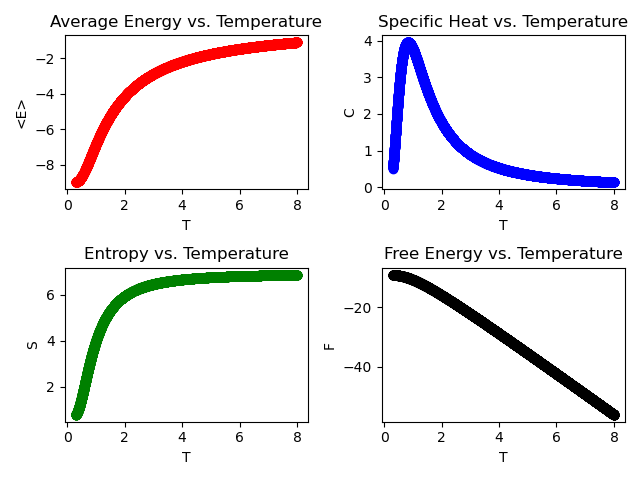
\includegraphics[width=0.75\textwidth]{../code/phy112l_lab3/3-4.png}
    \caption{Plot of average energy, specific heat, entropy, and free energy vs. temperature ($J = 1, N = 10$).}
    \label{fig:fig1}
\end{figure}
\clearpage

\problem
\subsection*{Part (a)}
At low temperatures, only the lowest energy state is accessible. There are two microstates where the system is in the state (all up and all down), so as $T \to 0$, $S \to \ln 2 \approx 0.693$.

\subsection*{Part (b)}
At high temperatures, all microstates are equally accessible, so the system tends towards the macrostate with the highest multiplicity, which is the one with equal numbers up and down, so as $T \to \infty$, $S \to \ln 2^{10} = 10\ln 2 \approx 6.931$. 

\subsection*{Part (c)}
At low temperatures, only the lowest energy state is accessible. The lowest energy states both have energy $-9$, so as $T \to 0$, $\langle E \rangle \to \frac{-9 + -9}{2} = -9$. At high temperatures, all microstates are equally accessible, so the average energy is the average of the energy of every accessible microstate. For a given microstate, we note that the microstate obtained from switching the spin of every even numbered site has an energy equal in magnitude and opposite in sign, as every alignment has been reversed (parallel alignments become antiparallel, and vice versa). Further, this microstate is unique, as if two microstates have the same corresponding microstate, applying the even-numbered switching transformation should yield the original microstate, which implies that the two microstates are the same. Consequently, every microstate has a unique corresponding microstate with equal and opposite energy, and by pairing those microstates when summing the energies of every microstate, we see that the total energy summed across microstates is zero, so as $T \to \infty$, $\langle E \rangle \to 0$. 

\end{document}